\documentclass[main.tex]{subfiles}

\newcommand\gauss[2]{1/(#2*sqrt(2*pi))*exp(-((x-#1)^2)/(2*#2^2))} % Gauss function, parameters mu and sigma
\begin{document}
\section{Introduction}
\paragraph{Objectif}: Présenter quelques élements  de la théorue de l'estimation statistique.
\subsection{Problématique}

\begin{figure}[H]
  \centering
  \begin{tikzpicture}
  \node[draw, ellipse] (P) at (0,0) {
    \begin{tabular}{c}
paramètres \\$\theta = \vect{\theta_1\\ \vdots\\\theta_n}$
    \end{tabular}};
  \node[draw, ellipse] (O) at (5,4) {
    \begin{tabular}{c}
      Observation \\
      Y=$g(\theta)$
    \end{tabular}};
  \node[draw, ellipse] (E) at (10,0){
    \begin{tabular}{c}
      Estimée\\
      $\hat{\theta} = h(y)$
    \end{tabular}};
  \draw[->,>=latex] (P) to[out=90, in = 180] (O);
  \draw[->,>=latex] (O) to[out=0, in=90] node[near end,left]{
    \begin{tabular}{c}
      Information à priori\\
      + Critère
    \end{tabular}}
      (E);
\end{tikzpicture}
\caption{Méthode d'estimation classique}
\end{figure}

Le raisonnement se transpose alors sur la figure suivante:
\begin{figure}[H]
  \centering
  \begin{tikzpicture}
    \draw[->,>=latex] (0,2) node{$\bullet$}node[right](theta){$\theta$} -- node[midway,left]{$\tilde{\theta}$}(-0.5,0) node{$\bullet$}node[right](hat){$\hat{\theta}$} ;
    \node[draw,ellipse,fit= (theta) (hat)](par) {};
    \node[below=5em] at (par) {\emph{Espace des paramètres}};
    \node (y) at (5,2) {$\bullet$~$y$};
    \node[draw,ellipse,minimum height=4cm,minimum width=2cm] (obs) at (5,1){};
    \node[below=5em] at (obs){\emph{Espace des observations}};
    \draw[->,>=latex] (theta) to[out=60, in=120] node[midway,above]{\emph{observation}} (y);
    \draw[->,>=latex] (y) to[out=-120,in=30,bend left] node[midway,below=0.5em]{\emph{estimation}}(hat);

  \end{tikzpicture}
  \caption{Raisonnement en espace algébrique}
\end{figure}


On défini les index suivants:
\begin{description}
\item[m] nombre d'expérience réalisée (taille de $y$)
\item[n] nombre de paramètres (taille de $\theta$)
\end{description}
\paragraph{Estimateurs statistiques}
On observe une réalisation $y= g(\theta)$ où $\theta$ est une VA. et on détermine $\hat{\theta} = h(Y)$ estimée.

\paragraph{Exemple}
\subparagraph{Exemple 1}$\Theta$ tension constante.\\
$y(t) = \theta +b(t)$. soit $y_i = \theta + b_i$\\
On défini donc $Y$ et $\Theta$ VA  et on a $Y = A\Theta + B$ -> régression linéaire.
\subparagraph{Exemple 2} filtre $RC$ $y(t) = (1-e^{-t/\tau})u(t)+b(t)$ , $\Theta=\tau$. modèle non linéaire, traité en TD.

\subsection{Performance-Qualité d'une estimation}
\begin{prop}[Grandeurs utiles]
  \begin{itemize}
  \item erreur d'estimation
    \[
      \tilde{\theta} = \hat{\theta}-\theta
    \]
  \item moment d'ordre 1:
\[
E_{Y|\Theta}[\tilde{\theta}]= E_{Y|\Theta}[\hat{\theta}]-\theta
\]
\item Biais moyen :
  \[
    E[\tilde{\theta}] = E_{Y\Theta}[\tilde{\theta}] = E[\hat{\theta}]-\theta
  \]
\item moment d'ordre 2:
  \begin{itemize}
  \item covariance de l'erreur d'estimation
    \[
      C_{\tilde{\theta}\tilde{\theta}} = E[(\tilde{\theta}-m_{\tilde{\theta}})(.)^T]
    \]
  \item Corrélation de l'erreur d'estimation
    \[
      \Gamma_{\tilde{\theta}\tilde{\theta}} = E[\tilde{\theta}\tilde{\theta}^T]
    \]
  \item Puissance :(Estimateur Quadratique moyen)
    \[
      P_{\tilde{\theta}} = E[\| \tilde{\theta}\|^2] = tr(\Gamma_{\tilde{\theta}\tilde{\theta}})
    \]
  \end{itemize}
  \end{itemize}
\end{prop}
\subsection{Caractérisation des estimateurs}
\begin{defin}
  \begin{itemize}
  \item Borne de Cramer Rao:
    borne minimale du biais de variance (qui dépend de l'estimateur choisi)
  \item Estimateur non biaisé: $E[\tilde{\theta}] = 0$
  \item Estimateur efficace: Borne de Cramer-Rao atteinte.
  \item Estimateur consistent: $E[\tilde{\theta}]\xrightarrow[N_{obs}\to\infty]{}0$ et $V[\tilde{\theta}]\xrightarrow[N_{obs}\to\infty]{}0$
  \item Estimateur robuste:\\ Les performances de l'estimateur ne sont pas trop dégradé si on s'écarte un peu des hypothèses sous laquelle l'estimateur a été établi.
  \item Complexité de l'estimateur:\\
    sur l'o btention des connaissances et mise en oeuvre de l'estimateur.
  \end{itemize}
\end{defin}
\section{Théorie classique de l'estimation}
\subsection{Estimateur des moindres carrés}
\begin{defin}
  Pour $Y$ une VA de moyenne $m_y =m_{Y|\theta}$ on défini le critère :
  \[
    J_{MC} = (Y-m_y)^TM(Y-m_y)
  \]
  Avec $M$ matrice symétrique définie positive
  et alors:
   \[
\hat{\theta}_{MC} = \arg\min_{\theta} J_{MC}(Y,\theta)
   \]
\end{defin}

\subsubsection{Condition nécessaire d'existance}

Si  $J_{MC}(y,\theta)$ est dérivable et pas de contrainte sur $\theta$.
\[
  \left.\nabla_J(\theta)\right|_{\hat{\theta}_{MC}} = \derivp[J_{MC}]{\theta} = 0 \quad \text{ Gradien}
\]

Il faut ensuite vérifié que c'est un minimum absolu:

\[
 \nabla^2_{J}(\theta) = \derivp[{}^2J_{MC}]{\theta\partial\theta^T} > 0 \quad \text{Hessien}
\]


\paragraph{Application}  $Y = A\theta{} + B$, avec $B$ une VA.
le critère des moindres carrés est alors :
\[
J_{MC} = (Y-A\theta-m_B)^TM (Y-A\theta-m_B)
\]
On a une forme quadratique  positive  car $A^TMA \geq0 $. (dans le cas $>0$  on a une CNS sur ce qui suit)
\subparagraph{Méthode 1}
\[
  \left.\nabla_J(\theta)\right|_{\hat{\theta}_{MC}} = 0  = -2 A^TM(Y-A\theta-m_B)
\]
Donc
\[
A^TMA \theta = A^TM(Y-m_B)
\]
Soit \[
  \boxed{\hat{\theta}_{MC} = \underbrace{(A^TMA)^{-1}AM}_{D}(Y-m_B)}
\]
On remarque que $DA = I_n$.
\subparagraph{Méthode 2} Pour $A^TMA>0$.

\[
  \begin{aligned}
    J_{MC} &= \underbracket{(D(Y-m_B)-\Theta)^TA^TMA(D(Y-m_B)-\theta)}_ {J_1(Y,\theta)}\\
    &+ \underbracket{(Y-m_B)^T(M-D^TA^TMAD)(Y-m_B)}_{J_2(Y)}
\end{aligned}
\]
Alors $\nabla J_{MC} = 0  \implies J_1 = 0 \implies D(Y-m_B) = \hat{\theta}_{MC}$


\subsubsection{Caractéristique de l'estimateur}
\begin{itemize}
\item Estimateur non biaisé

  \begin{align*}
    \tilde{\theta}_{MC} &=\hat{\Theta}-\theta\\
                   &= D(Y-m_B)-\theta \\
                   &= D(B-m_B)
  \end{align*}
Donc $E[\hat{\theta_{MC}}] = 0 $
\item moment d'ordre 2 :
  \[
      C_{\tilde{\theta}\tilde{\theta}} = E[(\tilde{\theta}-m_{\tilde{\theta}})(.)^T] = D E[(B-m_B)(B-m_B)^T]D^T = D C_{BB}D^T
    \]
    \begin{itemize}
    \item Cas MC ordinaire ($M=I_n$)
      \[
              C_{\tilde{\theta}\tilde{\theta}} = (A^TA)^{-1}A^TC_{BB}A(A^TA)^{-1}
      \]
    \item Cas MC pondéré ($M = C_{BB}^{-1}$)
      \[
        C_{\tilde{\theta}\tilde{\theta}} = (A^TC_{BB}^{-1}A)^{-1}
      \]
    \end{itemize}
  \item Cas $\theta$ scalaire $Y_i = \theta +B_i$ donc :
     \[
       C_{BB} =
       \begin{bmatrix}
         \sigma_1^2 &  &0 \\
         & \ddots &  \\
         0 & & \sigma_m^2
       \end{bmatrix} \text{ et }A = \vect{1\\ \vdots \\ 1}
     \]
     \begin{itemize}
     \item Cas MCO : $A^TA = m $
       \[
         \hat{\theta_{MC}} =\frac{\Sigma(y_i-m_{bi})}{m} \quad \text{ et } \quad \sigma_{\tilde{\theta}}^2 = \frac{\Sigma\sigma_i^2}{m^2}
       \]
     \item cas MCP pour $M = C_{BB}^{-1} = diag(\sigma_1^{-2}, \dots, \sigma_m^{-2})$
\[
  A^TC_{BB}A  = \sum_{i=1}^m \frac{1}{\sigma_i^2} \quad \text{ donc } \quad \hat{\theta}_{MCP} = \frac{1}{\sum \frac{1}{\sigma_i^2}}\sum_{}^{}\frac{Y_i-mB_i}{\sigma_i^2}
\]
\begin{itemize}
\item $\hat{\theta_{MCP}}$ défini un barycentre
\item Pour $\sigma_i = \sigma$ on a $M=\sigma I \implies MCO =MCP $
\end{itemize}

\end{itemize}
\item Comparaison MCO et MCP (avec $M = C_{BB}$)
  \begin{align*}
    \sigma_{MCO}^2 &\leq \sigma_{MCP}^2\\
    \frac{1}{\sum\sigma_i^{-2}} & \leq \frac{1}{m^2}\sum\sigma_i^2\\
    m ^2 &\leq \frac{1}{\sum\sigma_i^{-2}} \sum\sigma_i^2
  \end{align*}

\end{itemize}

\subsection{Estimateur du maximum de vraisemblance}
\begin{defin}
On considère $f_{Y}(y)$ ddp de $y$ paramétrée par $\theta$. On a $f_{Y|\theta}(y) = V(Y,\theta)$. on pose également $L(Y,\theta) = \ln(V(Y,\theta))$.

on défini alors:
\[
\hat{\theta}_{MV} = \arg\min f_{Y|\theta}(y) = \arg\min L(Y,\theta)
\]
\end{defin}

GRAPHE

\paragraph{Exemple} Modèle avec bruit additif gaussien.


\begin{prop}
  Dans le cas d'un brui Gaussien et pour $M = C_{BB}^{-1}$
  \[
    \hat{\theta}_{MCP}=\hat{\theta}_{MV}
  \]

\end{prop}

\paragraph{Remarque}
L'estimateur de MV n'est pas nécessairement efficace mais si un estimateur sans biais existe et est efficace c'est celui-ci.

Si $m \to\infty $ on montre que le MV est asymptotiquement efficace. (loi des grands nombres)
\section{Théorie générale de l'estimation}
\subsection{Estimateur linéaire en moyenne quadratique (ELMQ)}

\begin{defin}
  Un ELMQ fourni une estimée de la forme
  \[
   \hat{\theta} = HY +C
 \]
  à partir de l'erreur quadratique moyenne $E[\|\tilde{\theta}\|^2] = E[\tilde{\theta}\tilde{\theta}^T] =P_{\tilde{\theta}}$
\end{defin}
\paragraph{Concept} $H$ et $C$ tel que $P_{\tilde{\theta}}$ minimal.
\[
(1) \quad  \derivp[P_{\tilde{\theta}}]{H} = 0 \quad\text{ et }\quad (2)\quad \derivp[P_{\tilde{\theta}}]{C} = 0
\]
\begin{enumerate}[label=\arabic*)]
\item

  \begin{prop}
  \[
    \derivp[P_{\tilde{\theta}}]{H} =2E[HY+C-\theta] = 2E[\tilde{\theta}] = 0
  \]
    L'ELMQ est un estimateur non biaisé.
  \end{prop}
  et donc :
  \begin{align*}
    C &= -Hm_Y+m_\theta\\
    \hat{\theta} &= H(Y-m_y)+m_\theta \\
    \tilde{\theta} &= H(Y-m_y) - (\theta-m_\theta)
  \end{align*}

\item
  \begin{prop}
      \[
    \derivp[P_{\tilde{\theta}}]{C} =2E[(HY+C-\theta)Y^T] = 2E[\tilde{\theta}Y^T] = 0
  \]
  $\tilde{\theta} \perp Y $ quand la puissance est minimale, $\tilde{\theta}$ et $Y$ sont décorrélées, on a extrait toute l'information commune.
  \end{prop}
  \begin{figure}[H]\centering

  \begin{tikzpicture}
    \draw (-1,0,4.2) -- ++(0,0,-7) -- ++(5,0,0) -- ++(0,0,7) -- ++(-5,0,0)node[above,left]{\emph{
        \begin{tabular}{c}
          sous espace \\
          d'observation
        \end{tabular}}};
    \draw[->,>=latex] (1,0,3) -- (1,0,1) node[left]{$y_1$};
    \draw[->,>=latex] (1,0,3) -- (2,0,3) node[below]{$y_2$};
    \draw[->,>=latex] (1,0,3) -- (2,0,2) node[right]{$\hat{\theta}$};
    \draw[dashed] (2,0,2) -- node[midway,right]{$\tilde{\theta}$} (2,3,2)node{$\times$} node[above]{$\theta$};
  \end{tikzpicture}
  \caption{Représentation des paramètres}
\end{figure}
  De plus :
  \begin{align*}
    E[\tilde{\theta}Y^T]& =E[\tilde{\theta}(Y-m_Y)^T] \\
                   &= E[(H(Y-m_Y)-\theta-m_\theta)(Y-m_y)^T]\\
                   &= HC_{yy}-C_{\theta Y} = 0 \implies H = C_{\theta Y}C_{YY}^{-1}
  \end{align*}

  on a donc
  \[
    \boxed{\hat{\theta}=C_{\theta Y}C_{YY}^{-1}(Y-m_Y)+m_\theta}
  \]

  \paragraph{Remarque} L'ELMQ nécessite des connaissances du premier et du second ordre sur $\theta$ et $Y$.

  \begin{prop}
   \[
     C_{\tilde{\theta}\tilde{\theta}} = C_{\theta\theta}-C_{\theta Y}C_{YY}^{-1}C_{Y\theta}
   \]
   La corrélation entre $\theta$ et $Y$ permet de diminuer l'ELMQ.
 \end{prop}
\end{enumerate}


\subsection{Estimateur Bayésiens}
\subsubsection{Fonction coût/pénalité}
\begin{defin}
  On appelle fonction de coût ou fonction de pénalité une fonction qui mesure l'erreur entrainée par la prise de la valeur $\hat{\theta}$ pour $\theta$.
  \[
    C(\hat{\theta},\theta) \geq 0 \quad \text{ ou encore }\quad C(\tilde{\theta}) \ge 0
  \]
  On prendra le plus souvent une \og bonne \fg{} fonction (continue, paire , croissante ...)
\end{defin}

\paragraph{Exemple de coût} on représente les fonctions de coût usuelles:

\begin{figure}[H]
  \centering
  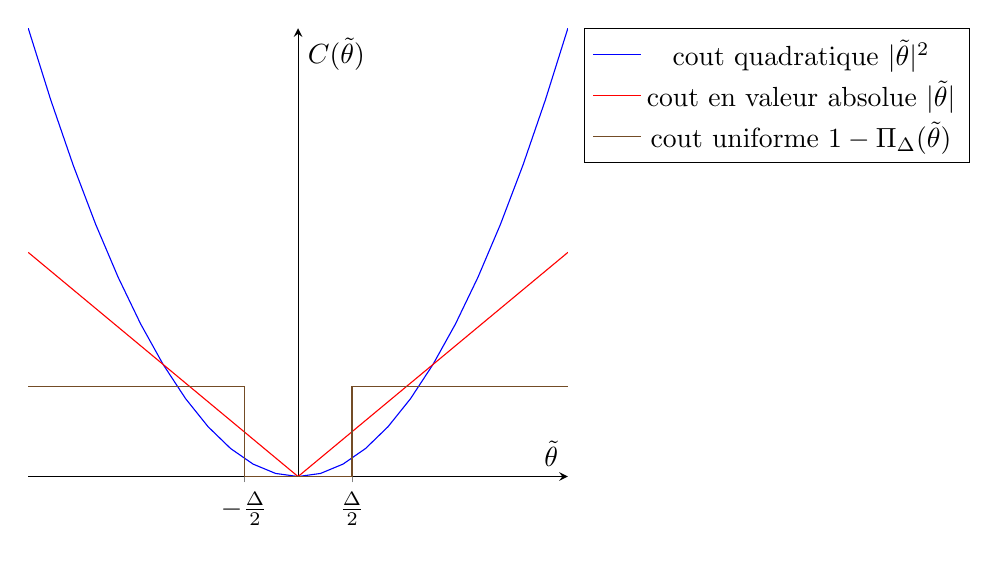
\begin{tikzpicture}
    \begin{axis}[axis lines=middle,
      xlabel={$\tilde{\theta}$},
      ylabel={$C(\tilde{\theta})$},
      ytick={0},
      ymax=20,
      xtick={-1,1},
      xticklabels={$-\frac{\Delta}{2}$,$\frac{\Delta}{2}$},
      legend pos=outer north east
      ]
      \addplot+[no marks]{0.8*x^2};
      \addlegendentry{cout quadratique $|\tilde{\theta}|^2$}
      \addplot+[no marks]{2*abs(x)};
      \addlegendentry{cout en valeur absolue $|\tilde{\theta}|$}
      \addplot+[no marks] coordinates{(-5,4)(-1,4)(-1,0)(1,0)(1,4)(5,4)};
      \addlegendentry{cout uniforme $1 -\Pi_\Delta(\tilde{\theta})$}
    \end{axis}
  \end{tikzpicture}
  \caption{Représentation des fonctions de coût classique}
\end{figure}

\begin{defin}
  On appelle estimateur bayésiens l'estimateur qui minimise le coût moyen :
  \begin{align*}
    E_{\theta,Y}[C(\hat{\theta},\theta)] &= \int_{\R^{m+n}}C(\hat{\theta},\theta)f_{\theta Y}(\theta,y)d\theta dy\\ &=\int_{\R^m}\left(\underbrace{\int_{\R^n}C(\hat{\theta},\theta)f_{\theta|Y=y}(\theta)d\theta}_{E_{\theta|Y}[C(\hat{\theta},\theta)]}\right) f_{Y}(y)dy
  \end{align*}
On minimise donc $ E_{\theta|Y}[C(\hat{\theta},\theta)]$ à coût conditionnel donné
  \[
    \hat{\theta}_{B} = \arg\min_{\hat{\theta}}E_{\theta|Y}[C(\hat{\theta},\theta)]
  \]
\end{defin}

\subsubsection{Estimateur du maximum a posteriori (MAP)}

On considère un cout uniforme.
\begin{defin}
  En prenant:
  \begin{align*}
    E_{\theta|Y}[C(\hat{\theta},\theta)] &= \int_{\R^m}(1-\Pi_{\Delta}(\tilde{\theta}))f_{\theta|Y=y}(\theta)d\theta \\
    &= 1 - \int_{\hat{\theta}-\Delta/2}^{{\hat{\theta}+\Delta/2}}f_{\theta|Y=y}(\theta)d\theta \\
      &\simeq 1- \Delta^nf_{\theta|Y=y}(\hat{\theta})
  \end{align*}
  Soit \[
    \hat{\theta}_{MAP}=\arg\max_{\theta} f_{\theta|Y=y}(\theta)
  \]
\end{defin}

\paragraph{Lien MAP-MV}

on a  $f_{\theta|Y=y}(\theta) f_{Y}(y) = f_{\theta Y}(\theta,y)$. Avec $f_\theta(\theta) = C^{ste}$ quand $f_{\theta Y}(\theta,y)$ à une valeur significative (ie $C_{\theta\theta}$ grand / $\sigma_\theta$  grand ) alors :
 \[
\arg\max f_{\theta|Y=y}(\theta) \simeq \arg\max f_{Y|\Theta=\theta}(y)
 \]

 On considère alors que $\theta$ est un paramètre  aléatoire mais très mal connu. (ddp uniforme sur un interval tres grand, peu d'infos sur $\theta$).

\emph{cf. TD \og file d'attente\fg{}}

\paragraph{Exemple et Application}

On considère $\theta$ scalaire aléatoire avec: $Y_i = \theta +B_i$ Avec :

$
\begin{cases}
B \hookrightarrow  \mathcal{N}(0,C_{BB})\\
\Theta \hookrightarrow\mathcal{N}(m_\theta,\sigma_\theta^2) \\
B \perp \Theta
\end{cases}$

\subparagraph{Rappel} MC=MV avec:
$\begin{cases}
m_B=0\\
\hat{\theta}_{MV} =\hat{\theta}_{MC} = \frac{\sum_{i=1}^{m}Y_i}{m}\\

E[\hat{\theta}_{MV}] = E[\theta]=m_\theta \text{ et } \sigma_{\tilde{\theta}_{MV}}=\frac{\sigma_B}{m}\\
\end{cases}$

On a donc:
\[
  f_{Y|\theta}(y)=f_{B}(Y-A\theta) = \prod_{i=1}^{m}f_{B_i}(Y_i-\theta) = C_1 \exp\left(-\frac{1}{2}\frac{\sum(Y_i-\theta)^2}{\sigma_B^2}\right)
\]
Or
\[
  f_{\theta|Y=y}(\theta) = \frac{f_{Y|\theta}(y)f_\theta(\theta)}{f_Y(y)} = C_2 \exp\left(-\frac{1}{2}\underbrace{\left[\frac{\sum(Y_i-\theta)^2}{\sigma_B^2}+\frac{(\theta-m_\theta)^2}{\sigma_\theta^2}\right]}_{J_{MAP}}\right)
\]
Le critère est ici une forme quadratique, donc :

\[
  \hat{\theta}_{MAP} = \arg\max f_{\theta|Y=y}(\theta)  = \arg\min J_{MAP}(\theta,Y)
\]
Alors on a la CNS :
\[
\deriv[J_{MAP}]{\theta} = 0 = 2 \left[ -\sum_{i=1}^{m}\frac{Y_i-\theta}{\sigma_b^2}+\frac{(\theta-m_\theta)^2}{\sigma_\theta^2}\right]
\]
Soit une expression barycentrique :
\[
  \hat{\theta}_{MAP} = \frac{\frac{m}{\sigma_B^2}\sum_{}^{}\frac{Y_i}{m}+\frac{m_\theta}{\sigma_\theta^2}}{\frac{m}{\sigma_B^2}+\frac{1}{\sigma_\theta^2}}
\]
Donc :
\begin{prop}
\[
E[\hat{\theta}_{MAP}]  = m_\theta
\]
L'estimateur est non biaisé. De plus :
\[
  \sigma_{\tilde{\theta}_{MAP}}^2= \frac{1}{\frac{1}{\sigma_{MV}}+\frac{1}{\sigma_\theta^2}} <
  \begin{cases}
    \sigma_\theta^2 \\
    \sigma_{MV}^2
  \end{cases}
\]
On a fait mieux en prenant en compte toutes les sources d'informations.
\end{prop}

\paragraph{Remarque}
\begin{itemize}
\item Si $\sigma_\theta>>\sigma_{MV}$ alors $\hat{\theta}_{MAP}\simeq \hat{\theta}_{MV}$ (ce qui arrive pour $\sigma_B$ ou $m$ grand)
\item Si $\sigma_\theta<<\sigma_{MV}$ et $\hat{\theta}_{MAP} \simeq m_\theta$ (l'obersavation apporte peu d'info)
\end{itemize}

\subsubsection{Estimateur en moyenne quadratique (EQM)}

\begin{defin}
  On le cout moyen de l'EQM:
  \[
    C(\hat{\theta},\theta) = (\hat{\theta}-\theta)^T M (\hat{\theta}-\theta)
  \]
  Avec $M>0$.
  On cherche a minimiser le cout moyen mais sans contrainte de linéarité avec une matrice de pondération qui peux prendre en compte des facteurs d'echelles ou des unités différentes.
\end{defin}


\paragraph{Etude de l'estimateur} On veut minimiser $E_{\Theta|Y}[C(\hat{\theta},\theta)]$
\begin{align*}
  \nabla_{\hat{\theta}}E_{\Theta|Y}[C(\hat{\theta},\theta)] &= 0 \\
  E_{\theta|Y}[2M(\hat{\theta}-\theta)] &= 0 \\
  2M E_{\theta|Y}[\underbracket{\hat{\theta}}_{h(y)}]-E_{\theta|Y}[\theta]&=0 \\
  2M(\hat{\theta}-E_{\theta|Y}[\theta]) &= 0 \\
  \Aboxed{ \hat{\theta}_{MQ} &=E_{\theta|Y}[\theta]} \\
                          &= \int_{\R^n}\theta f_{\theta|y}(\theta)d\theta = h(Y=y)
\end{align*}

Par conséquent: $E[\hat{\theta}_{MQ}]=E[\theta]$. on a un estimateur non biaisé.
\paragraph{Remarque}
Si $f_{\theta|Y}$ possède un axe de symétrie (ex: gaussienne) :


FIGURE . ($\hat{\theta}_{MQ}=\hat{\theta}_{MAP}$ dans le cas gaussien. Différent avec deux bosses.)


Dans le cas général la contrainte de linéarité pour l'ELMQ conduit à une valeur plus grande qu'avec l'EQM. Dans le cas gaussien: $\hat{\theta}_{ELMQ}=\hat{\theta}_{MQ}$, mais $\hat{\theta}_{MQ}$ nécessite plus de connaissance (ddp).

\subsubsection{Estimateur en valeur absolu}

\begin{defin}
  on s'interesse au cas $n=1$ (un paramètre)
  On choisit le cout moyen :
  \[
    C(\hat{\theta},\theta) = |\hat{\theta}-\theta|
  \]
  Alors :
  \[
    E_{\theta|Y}[C(\hat{\theta},\theta)] = \int_{-\infty}^{\hat{\theta}}(\hat{\theta}-\theta)f_{\theta|Y=y}(\theta)d\theta-\int_{\hat{\theta}}^{+\infty}(\hat{\theta}-\theta)f_{\theta|Y=y}(\theta)d\theta
  \]
\end{defin}

Donc :
\begin{align*}
  0 =&  \nabla_{\hat{\theta}}E_{\theta|Y}[C(\hat{\theta},\theta)] \\
     =& \dots \\
     =&\int_{-\infty}^{\hat{\theta}}f_{\theta|Y=y}(\theta)d\theta-\int_{\hat{\theta}}^{+\infty}f_{\theta|Y=y}(\theta)d\theta
\end{align*}

\begin{prop}
  L'estimée est alors $\hat{\theta}_{VA}$ tel que :
  \[
    \int_{-\infty}^{\hat{\theta}}f_{\theta|Y=y}(\theta)d\theta = \int_{\hat{\theta}}^{+\infty}f_{\theta|Y=y}(\theta)d\theta
  \]
  On parle de médiane a posteriori. Le résultat se généralise pour tout $n$.
\end{prop}

\paragraph{Remarque} Dans le cas où $f_{\theta|Y=y}(\theta)$ possède un axe de symétrie (ex gaussienne) on a :
\[
  \hat{\theta}_{VA} =\hat{\theta}_{MV} \equals^{\stackrel{\max}{\downarrow}} \hat{\theta}_{MAP}
\]

\paragraph{Exemple} Localisation d'un véhicule / Ellipsoïde de confiance (cf poly).
\section{Conclusion}
\begin{itemize}
\item L'estimateur statistique dépend des connaissances a priori, de la complexité des calculs et de la robustesse attendue.
\item Dans certains cas particuliers/ limites on retrouve des estimateurs intuitifs /empirique.
\item La loi normale joue un rôle important (hypothèses qui se justifie par la loi des grands nombres): les calculs sont simplifiés et conduisent au même résultat.

\end{itemize}



\end{document}
